\documentclass[14pt]{extarticle}

\usepackage{geometry}
\geometry{a4paper,
          total={165mm,257mm},
          left=30mm,
          top=20mm,
         }

\usepackage[utf8]{inputenc}
\usepackage[T1, T2A]{fontenc}
\usepackage[english, russian]{babel}
\usepackage{csquotes}

\usepackage[
    backend = biber,
    style = numeric,
]{biblatex}

\addbibresource{Refs.bib}

\usepackage{graphicx}
\graphicspath{ {./images/} }

\usepackage{subcaption}

% \usepackage{amsmath}


\title{Моделирование частотных сканов}
\author{Богачев А.М.}
\date{\today}


\begin{document}

    \maketitle
    \begin{abstract}
        В отчёте приведены результаты моделирования частотных сканов,
        образованных сигналом релаксации, состоящим из трёх 
        экспоненциальных сигналов с единичной амплитудой. При моделировании
        не учитывается влияние шумов. Показано, что показатель 
        нелинейности"=неэкспоненциальности $p$ убывает с увеличением 
        разницы между постоянными времени крайних состоавляющих на спектре, 
        при этом растёт среднеквадратическая ошибка между результатами 
        измерений и результатами моделирования. В отчёте также приведена 
        математическая модель частотного скана и краткое описание её 
        программной реализации. В графическом виде приведены примеры 
        спектров, результатов идентификации модели; приведён график 
        зависимости $p$ от разности между постоянными времени крайних 
        составляющих на спектре, в приложении приведена таблица с 
        результатами моделирования частотных сканов.
    \end{abstract}
    \tableofcontents

    \pagebreak

    \chapter{Цели и задачи}

Согласно обзору \cite{istratov_exp_analysis} сигналы релаксации ёмкости 
барьерных структур можно условно разделить на три группы:
\begin{enumerate}
    \item Моноэкспоненциальный сигнал релаксации, обусловленный одним  
    энергетическим уровнем в запрещённой зоне полупроводника.
    \item Сигнал релаксации, состоящий из суммы нескольких моноэкспоненциальных 
    сигналов релаксации.
    \item Сигнал релаксации, характеризуемый непрерывным распределением скоростей 
    эмиссии, представленным спектральной функцией $g(\lambda)$.
\end{enumerate}

Таким образом, цель работы по моделированию частотных сканов можно описать 
следующим образом: найти способ определять спектральную функцию 
$g(\lambda)$, её параметры, а также зависимость этих параметров от температуры.

Для достижения поставленной цели нужно решить следующие задачи:
\begin{enumerate}
    \item Разработать алгоритм идентификации частотного скана 
    моноэкспоненциального сигнала релаксации.
    \item Разработать алгоритм идентификации частотного скана 
    неэкспоненциального сигнала релаксации с показателем $p$, 
    характеризующим нелинейность и неэкспоненциальность.
    \item Разработать программу идентификации частотного 
    скана сигнала релаксации, состоящего из суммы моноэкспоненциальных 
    сигналов. Программа должна определять параметры каждого 
    моноэкспоненциального сигнала.
    \item Разработать программу идентификации группы частотных сканов 
    при разных температурах. На данном этапе предполагается, что сигнал 
    релаксации образован суммой моноэкспоненциальных сигналов, 
    количество которых не меняется в зависимости от температуры, 
    меняются только их параметры.
    \item Разработать программу иденитификации спектральной 
    функции $g(\lambda)$ и её параметров для отдельного 
    частотного скана.
    \item Разработать программу иденитификации спектральной 
    функции $g(\lambda)$ и её параметров для группы частотных сканов при 
    разных температурах, полагая, что от температуры зависят только 
    параметры $g(\lambda)$.
\end{enumerate}

    \section{Математическе модели}

    В данном разделе представленно описание модели частотного скана 
    в математических выражениях.


    \subsection{Модель сигнала релаксации ёмкости}

    Согласно обзору \cite{istratov_exp_analysis}, зависимость значения
    ёмкости от времени $f(t)$ для моноэкспоненциального сигнала релаксации
    имеет вид выражения \ref{eq:monoexp}.
    \begin{equation}
        \label{eq:monoexp}
        f(t) = A \exp \left(-\lambda t\right) ,
    \end{equation}
    где
    \begin{description}
        \item[\(A\)] -- амплитуда сигнала релаксации ёмкости;
        \item[\(\lambda\)] -- скорость экспоненциального спада,
        обратнопрпорциональная постоянной веремени сигнала релаксации
        $\tau$ (выражение \ref{eq:lambda}).
    \end{description}
    \begin{equation}
        \label{eq:lambda}
        \lambda = \tau ^ {-1}
    \end{equation}
    Спектр моноэкспоненциального сигнала релаксации имеет вид, 
    представленный на рисунке \ref{pic:monoexp_spect_example}.
    \begin{figure}[ht]
        \centering
        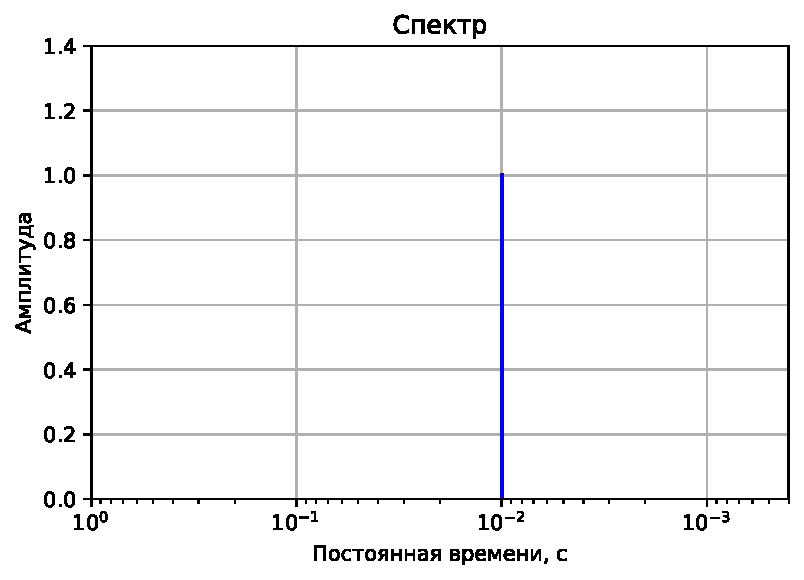
\includegraphics[width=0.5\textwidth]{monoexp_spect_expample}
        \caption{Пример спектра моноэкспоненциального сигнала релаксации
        ёмкости.}
        \label{pic:monoexp_spect_example}
    \end{figure}

    Согласно источнику \cite{istratov_exp_analysis}, зависимость сигнала 
    релаксации ёмкости от времени $f(t)$ для сгинала, образованного 
    несколькими дискретными экспоненциальными сигналами, определяется 
    выражением 
    \ref{eq:discr_multiexp}.
    \begin{equation}
        \label{eq:discr_multiexp}
        f(t) = \sum_{i=1}^{n}A_i\exp\left(-\lambda_i t\right) ,
    \end{equation}
    где $n$ -- количество экспоненциальных составляющих в спектре.
    Пример спектра такого сигнала показан на рисунке 
    \ref{pic:multiexp_spect_example}.
    \begin{figure}[ht]
        \centering
        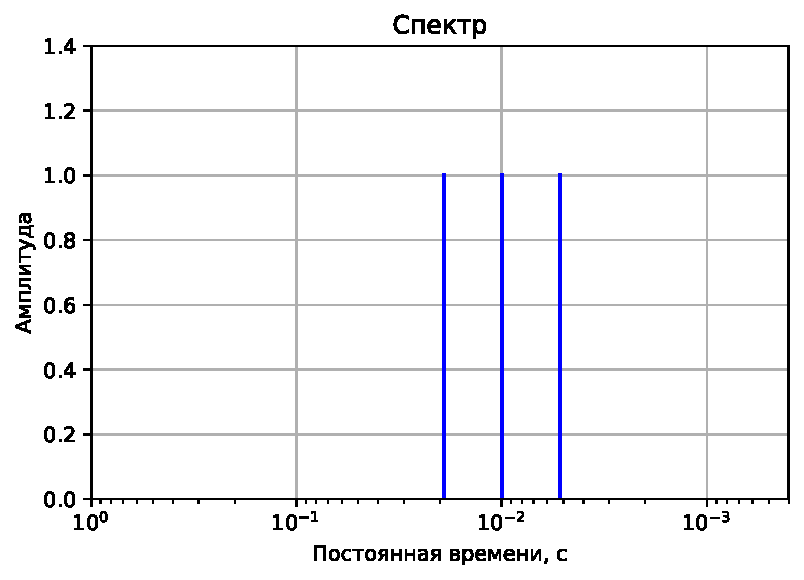
\includegraphics[width=0.5\textwidth]{multiexp_spect_example}
        \caption{Пример спектра сигнала релаксации ёмкости, содержащего
        несколько экспоненциальных составляющих.}
        \label{pic:multiexp_spect_example}
    \end{figure}


    \subsection{Модель аппаратных преобразований спектрометра DLS"~82E}

    В спектрометре DLS-82E реализована корреляционная обработка сигнала
    релаксации ёмкости, таким образом сигнал на выходе аналогового тракта
    спектрометра определяется выражением \ref{eq:dlts_correlation_tech},
    согласно публикации \cite{istratov_exp_analysis}.
    \begin{equation}
        \label{eq:dlts_correlation_tech}
        S\left[g(\lambda),t_c,t_d\right]=\frac{1}{t_c}\int_{t_d}^{t_d+t_c}
        f(t)W\left(t-t_d\right)dt ,
    \end{equation}
    где
    \begin{description}
        \item[$W(t)$] -- весовая функция, определённая на интервале 
        времени $\left[0,t_c\right]$,
        \item[$t_c$] -- период (длительность) весовой функции $W(t)$,
        \item[$t_d$] -- время задержки между началом сигнала релаксации
        и началом корреляционной обработки. Согласно обзору 
        \cite{istratov_exp_analysis}, время задержки $t_d$, обычно, 
        вводится для улучшения избирателности или для снижения искажения
        сигнала из-за перегрузки измерительной системы.
        \item[$g(\lambda)$] -- распределение скоростей экспоненциальных
        спадов, составляющих релаксационный сигнал.
    \end{description}

    Модель аппаратных преобразований (корреляционной обработки),
    учитывающая форму весовой функции, реализованной в спектрометре
    DLS"~82E, для моноэкспоненциального сигнала определяется выражением
    \ref{eq:dls82e_model_S} \cite{rp_vak}.
    \begin{equation}
        \label{eq:dls82e_model_S}
        S\left(\tau,C_A,F_0, t_1\right) = C_A K_{BS} K_{LS} 
        \phi\left(\tau,F_0,t_1\right),
    \end{equation}
    где
    \begin{description}
        \item[$C_A$] -- амплитуда емкостного релаксационного сигнала,
        \item[$K_{BS}$] -- масштабный коэффициент, зависящий от 
        чувствительности емкостного моста,
        \item[$K_{LS}$] -- масштабный коэффициент селектора,
        \item[$\tau$] -- постоянная времени релаксации гулбокого уровня,
        \item[$F_0$] -- частота сканирования импульсов заполнения,
        \item[$t_1$] -- длительность импульса заполнения,
        \item[$\phi\left(\tau,F_0,t_1\right)$] -- функция определяемая
        выражением \ref{eq:dls82e_model_phi}.
    \end{description}
    \begin{equation}
        \label{eq:dls82e_model_phi}
        \phi\left(\tau,F_0,t_1\right) = 
        M \tau F_0 e^{-\frac{0.05}{\tau F_0}}
        \left(1-e^{\frac{t_1 F_0-0.45}{\tau F_0}}
        -e^{-\frac{0.5}{\tau F_0}}+
        e^{\frac{t_1 F_0-0.95}{\tau F_0}}\right),
    \end{equation}
    где $M$ -- масштабный множитель.

    Масштабный множитель $M$ определяется выражением
    \ref{eq:dls82e_model_M}.
    \begin{equation}
        \label{eq:dls82e_model_M}
        M(\tau, F_0, t_1) = \frac{1}{\max{\left[
        \tau F_0 e^{-\frac{0.05}{\tau F_0}}
        \left(1-e^{\frac{t_1 F_0-0.45}{\tau F_0}}
        -e^{-\frac{0.5}{\tau F_0}}+
        e^{\frac{t_1 F_0-0.95}{\tau F_0}}\right)
        \right]}}
    \end{equation}

    Введём коэффициент $A$ (выражение \ref{eq:dls82e_model_A}), 
    характеризующий амплитуду сигнала релаксации ёмкости и перепишем 
    выражение \ref{eq:dls82e_model_S} с учётом того, что длительность
    импульса заполнения $t_1$ является неизменной величиной, и получим
    выражение \ref{eq:dls82e_model_S_short}.
    \begin{equation}
        \label{eq:dls82e_model_A}
        A = C_A K_{BS} K_{LS}.
    \end{equation}
    \begin{equation}
        \label{eq:dls82e_model_S_short}
        S(\tau,A,F_0) = A\phi(\tau, F_0)
    \end{equation}

    Для одновременного учёта нелинейности аппаратного тракта и 
    неэкспоненциальности сигнала релаксации, связанной с пресутствием 
    нескольких экспоненциальных составляющих в модель вводят коэффициент
    нелинейности"=неэкспоненциальности $p$ \cite{rp_vak}, после чего 
    выражение \ref{eq:dls82e_model_S_short} приобретает вид выражения 
    \ref{eq:dls82e_model_S_p}.
    \begin{equation}
        \label{eq:dls82e_model_S_p}
        S(\tau,A,F_0,p) = A\left[\phi(\tau, F_0)\right]^p.
    \end{equation}

    Для моноэкспоненциальных сигналов релаксации коэффициент $p=1$, но,
    как будет показано далее, в случае наличия нескольких экспоенециальных
    составляющих в сигнале релаксации коэффициент $p$ становится меньше~1.


    \subsection{Модель для расчёта исходных данных}
    Если предположить, что сигнал релаксации ёмкости состоит из нескольких
    экспоненциальных составляющих и определяется выражением
    \ref{eq:discr_multiexp}, то опираясь на выражения
    \ref{eq:discr_multiexp}, \ref{eq:dlts_correlation_tech}, 
    \ref{eq:dls82e_model_S_short} и \ref{eq:dls82e_model_phi}, можно
    сделать выод, что частотный скан, созданный таким сигналом релаксации
    ёмкости определяется выражением~\ref{eq:multiexp_frequncy_scan}.
    \begin{equation}
        \label{eq:multiexp_frequncy_scan}
        Y = \sum_{i=1}^{n} A_i \phi(\tau_i, F_0) ,
    \end{equation}
    где $n$ -- количество экспоненциальных составляющих в сигнале 
    релаксации.

    \section{Моделирование и его результаты}
	В данном разделе приводится краткое описание программной реализации
	модели, примеры рассчитанных частотных сканов, примеры результатов
	идентификации их моделей и график зависимости коэффициента 
	нелинейности"=неэкспоненциальности $p$ от расстояния между крайними
	линиями на спектре.

	\subsection{Реализация модели}
	Модель (выражение \ref{eq:dls82e_model_S_p}) реализована на 
	языке программирования Python (версия 3.9.12) с применением 
	библиотеки TensorFlow (версия 2.8.0) и других библиотек	для научных
	вычислений.

	Модель частотного скана реализованна в виде отдельного класса \\
	\emph{FrequencyScan()} в модуле \emph{fsmodels.py}. Код 
	прокомментирован. Все параметры снабжены адекватными значениями по 
	умолчанию. В дальнейшем планируется дополнение документации и 
	перенос всех программных инструментов для обработки 
	экспериментальных данных в один пакет.

	Модель реализует две функции:
	\begin{enumerate}
		\item Вычисление частотного скана по заданным параметрам и 
		заданному вектору десятичных логарифмов частот опорной функции.
		\item Идентификация параметров модели частотного скана по 
		экспериментальным данным.
	\end{enumerate}
	Имеется возможность вывода значений параметров модели на каждой 
	итерации при идентификации. Примеры использования модели можно найти
	в файле \emph{tensorflow\_model.ipynb} (ПО Jupyter Notebook в составе 
	дистрибутива Anaconda).

	Программа при каждом вычислении значения $\phi\left(\tau,F_0,
	t_1\right)$	(выражение~\ref{eq:dls82e_model_phi}) находит 
	\(
		\max{\left[
	    \tau F_0 e^{-\frac{0.05}{\tau F_0}}
	    \left(1-e^{\frac{t_1 F_0-0.45}{\tau F_0}}
	    -e^{-\frac{0.5}{\tau F_0}}+
	    e^{\frac{t_1 F_0-0.95}{\tau F_0}}\right)
	    \right]}
    \)
	методом	градиентного спуска и вычисляет масштабный множитель $M$ 
	(выражение \ref{eq:dls82e_model_M}).

	Идентификация параметров модели производится методом градиетного 
	спуска, при этом минимизируется среднеквадратическая ошибка между 
	значениями, полученными в результате измерений, и результатами 
	моделирования (выражение \ref{eq:mse}).
	\begin{equation}
		\label{eq:mse}
		E = \frac{1}{n}\sum_{i=1}^{n}\left(y_i - y_i^*\right)^2,
	\end{equation}
	где
	\begin{description}
		\item[$y_i$] -- значения, полученные в результате измерений,
		\item[$y_i^*$] -- значения, полученные в результате моделирования,
		\item[$n$] -- количество измерений.
	\end{description}

	Градиентный спуск везде реализован с помощью библиотеки TensorFlow,
	которая использует алгоритм дифференцирования на графе вычислений,
	таким образом, производная берётся символьно (точно), затем вычисляется
	её значение, поэтому точность вычисления градиента ограничена только
	разрядностью чисел \cite{hands_on_ml}.

	\textbf{Для ускорения процесса идентификации и улучшения сходимости
	в модели вместо постоянной времени сигнала релаксации $\tau$ 
	выполняется идентификация величины $\rho = \log_{10}(\tau)$. По этим же
	и некоторым	другим техническим причинам при вычислении частотного 
	скана на вход модели нужно подавать не вектор частот опорной 
	функции, а вектор их десятичных логарифмов.}

	На рисунке \ref{pic:identification_test} показан пример результата
	идентификации модели на тестовых (специально сгенерированных) данных.

	\begin{figure}[h!]
		\centering
		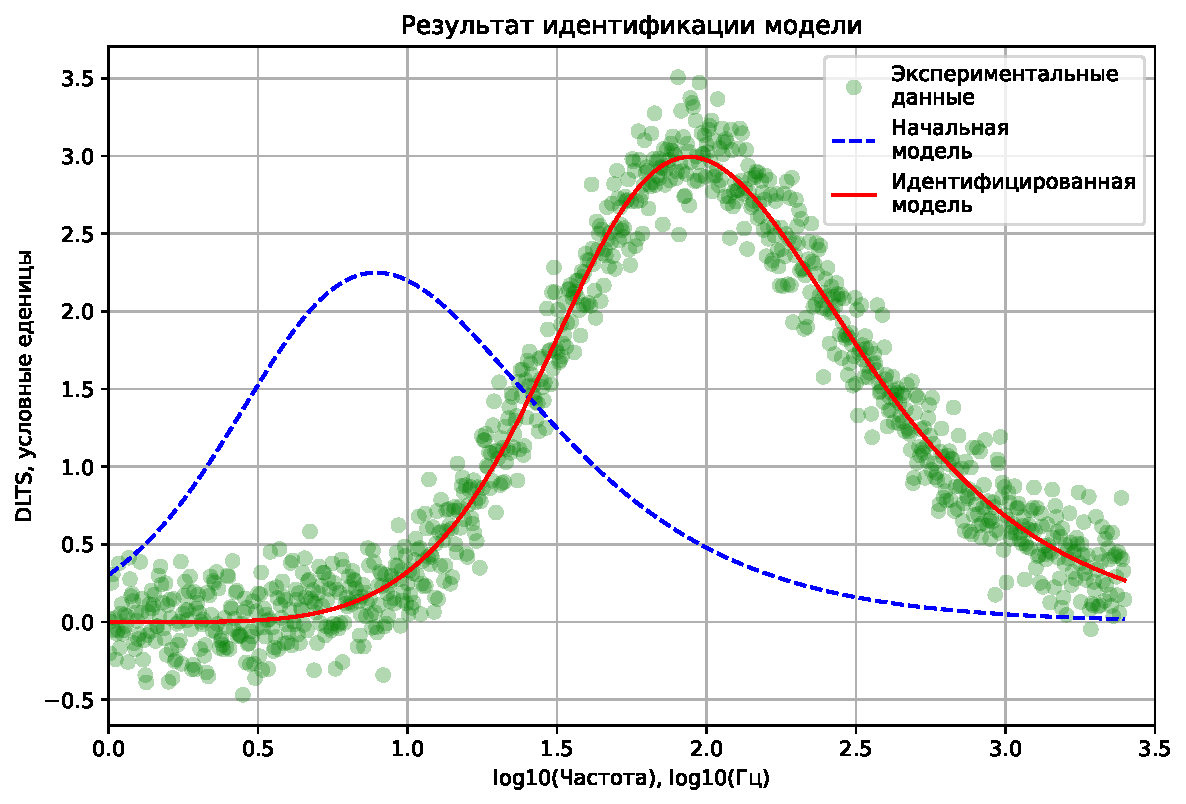
\includegraphics[width=0.75\textwidth]{identification_test}
		\caption{Пример результата идентификации модели.}
		\label{pic:identification_test}
	\end{figure}

	На рисунке \ref{pic:param_path} показан <<путь>> изменеия параметров 
	(десятичного логарифма постоянной времени и амплитуды) при
	идентификации. Красными точками отмечены значения параметров на 
	каждой итерации, изолинии показывают значения среднеквадратической
	ошибки. 

	В идеальном случае изолинии должны иметь форму концентрических
	окружностей, а <<траекторя>> значений параметров должна быть прямой
	линией (в случае обычного градиентного спуска), направленной к центру
	данных окружностей. Таким образом, рисунок \ref{pic:param_path} 
	позволяет сделать вывод о возможности повышения скорости идентификации.

	\begin{figure}[h!]
		\centering
		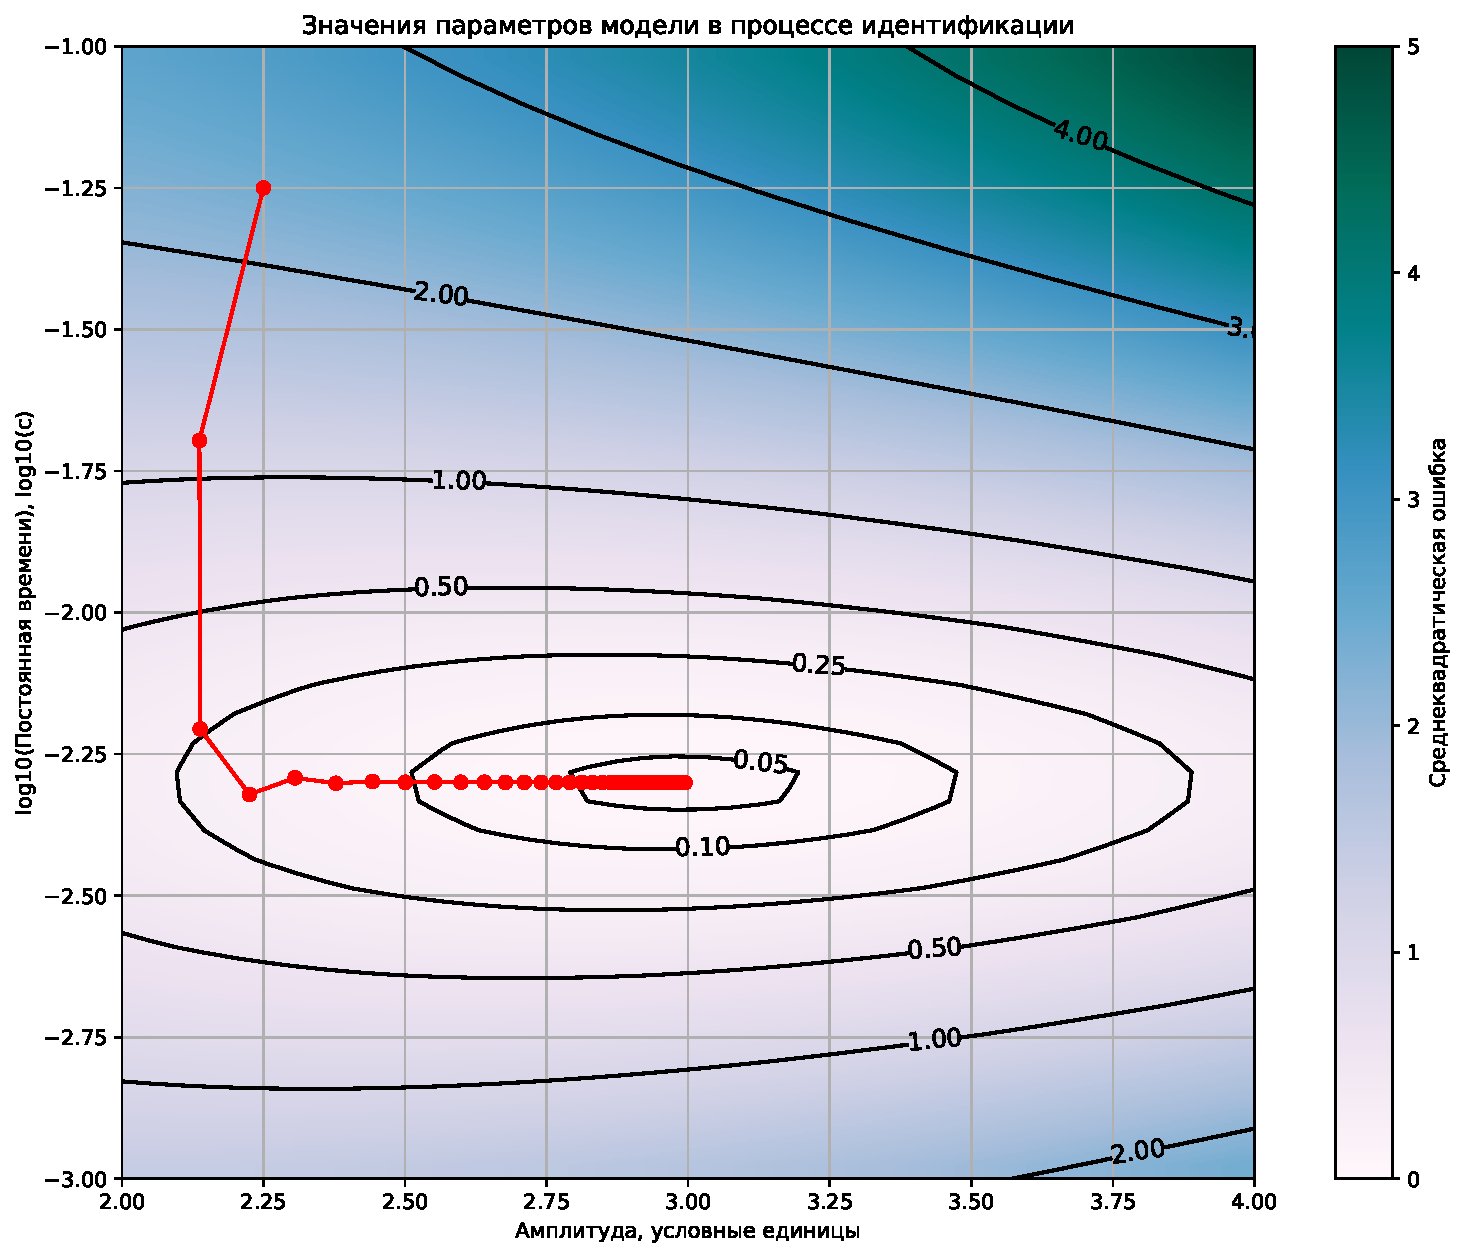
\includegraphics[width=0.75\textwidth]{path}
		\caption{<<Путь>> значений параметров при идентификации.}
		\label{pic:param_path}
	\end{figure}


	\subsection{Результаты моделирования}

	Для определения формы зависимости показателя 
	нелинейности"=неэкспоненциальности $p$ было вы полнено моделирование 
	31 частотного скана со спектрами, состоящими из трёх экспоненциальных
	составляющих единичной амплитуды. При моделировании предполагалось,
	что условия идеальны и частотные сканы не содержат шума.

	На первом этапе моделирования, соглассно выражению \ref{eq:multiexp_frequncy_scan},
	рассчитывался частотный скан, затем производилась идентификация 
	параметров модели этого частотного скана, согласно выражению 
	\ref{eq:dls82e_model_S_p}. Идентификация проводилась по всем точкам.

	Результаты моделирования некоторых частотных сканов и спектры, по 
	которым эти частотные сканы были рассчитаны, приведены на рисунках~
	\ref{pic:result_0},	\ref{pic:result_1}, \ref{pic:result_2}. 
	В таблице~\ref{table:results}, вынесенной в приложение приведены 
	полные результаты моделирования. На рисунке~\ref{pic:p_delta_tau} 
	показан график полученной зависимости показателя	
	нелинейности"=неэспоненциальности от разности постоянных времени
	крайних на спектре линий.

	\begin{figure}[h!]
		\centering
		\begin{subfigure}[c]{0.3\textwidth}
			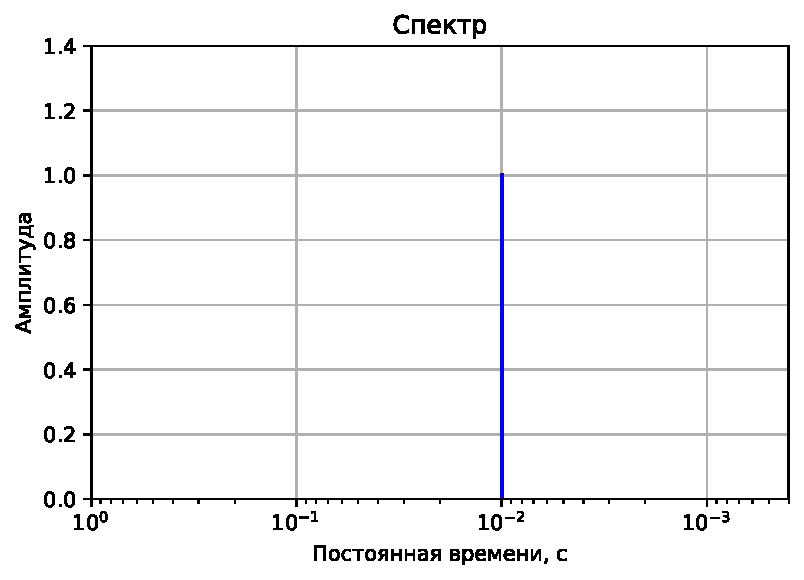
\includegraphics[width=\linewidth]{spectr0}
			\caption{Спектр}
			\label{pic:results_0_spectr}
		\end{subfigure}
		\begin{subfigure}[c]{0.4\textwidth}
			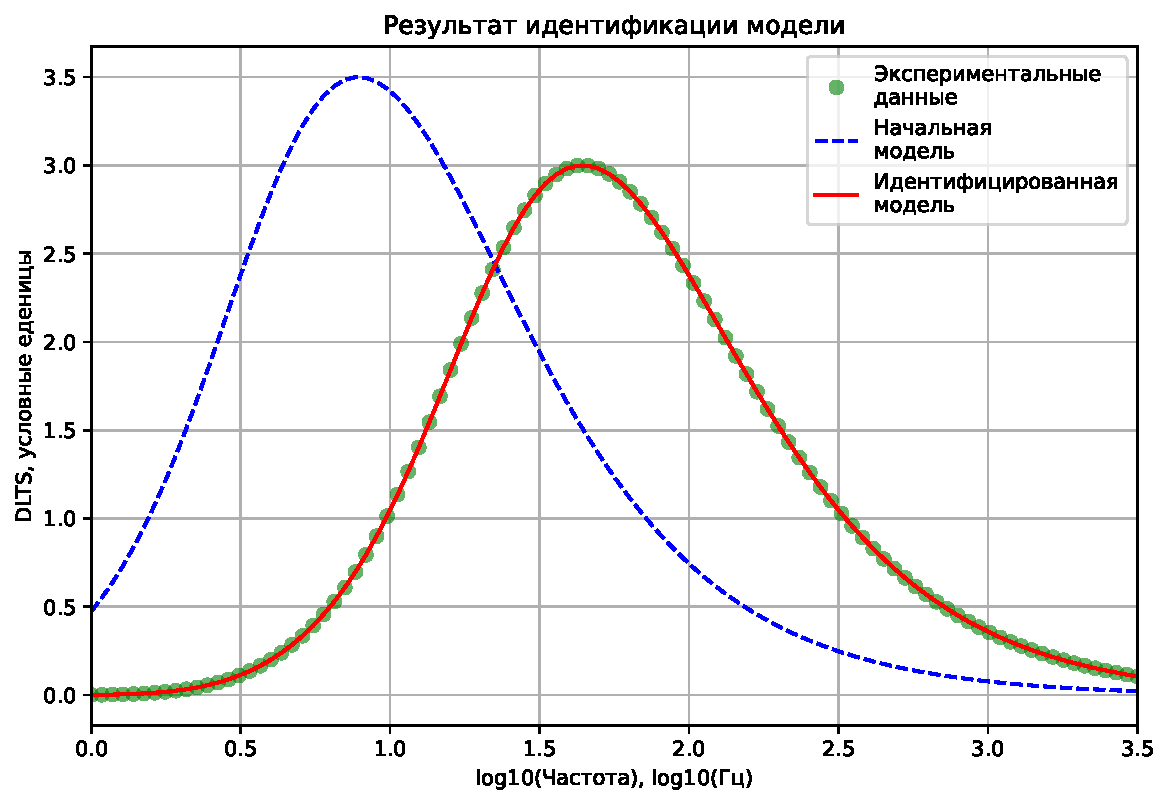
\includegraphics[width=\linewidth]{identification_results_0}
			\caption{Рассчитанный частотный скан и результаты идентификации}
			\label{pic:results_0_scan}
		\end{subfigure}
		\caption{Результаты моделирования частотного скана №1}
		\label{pic:result_0}
	\end{figure}

	\begin{figure}[h!]
		\centering
		\begin{subfigure}[c]{0.3\textwidth}
			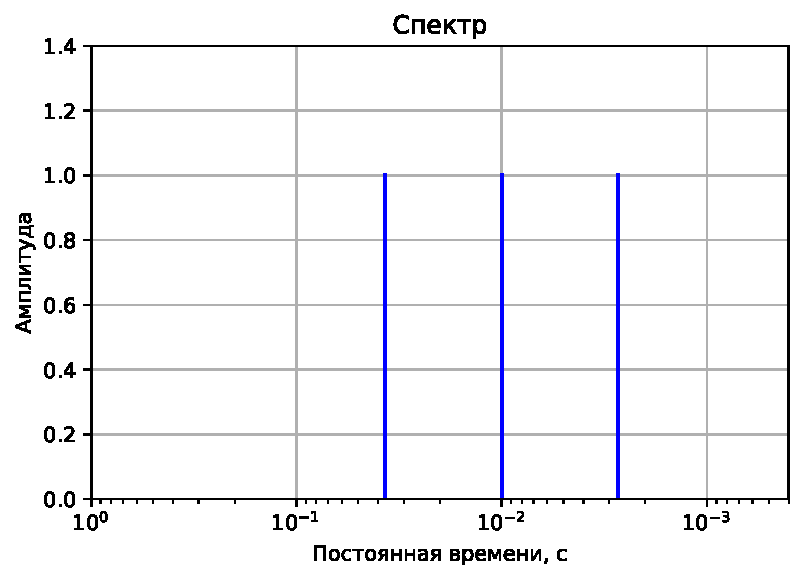
\includegraphics[width=\linewidth]{spectr17}
			\caption{Спектр}
			\label{pic:results_1_spectr}
		\end{subfigure}
		\begin{subfigure}[c]{0.4\textwidth}
			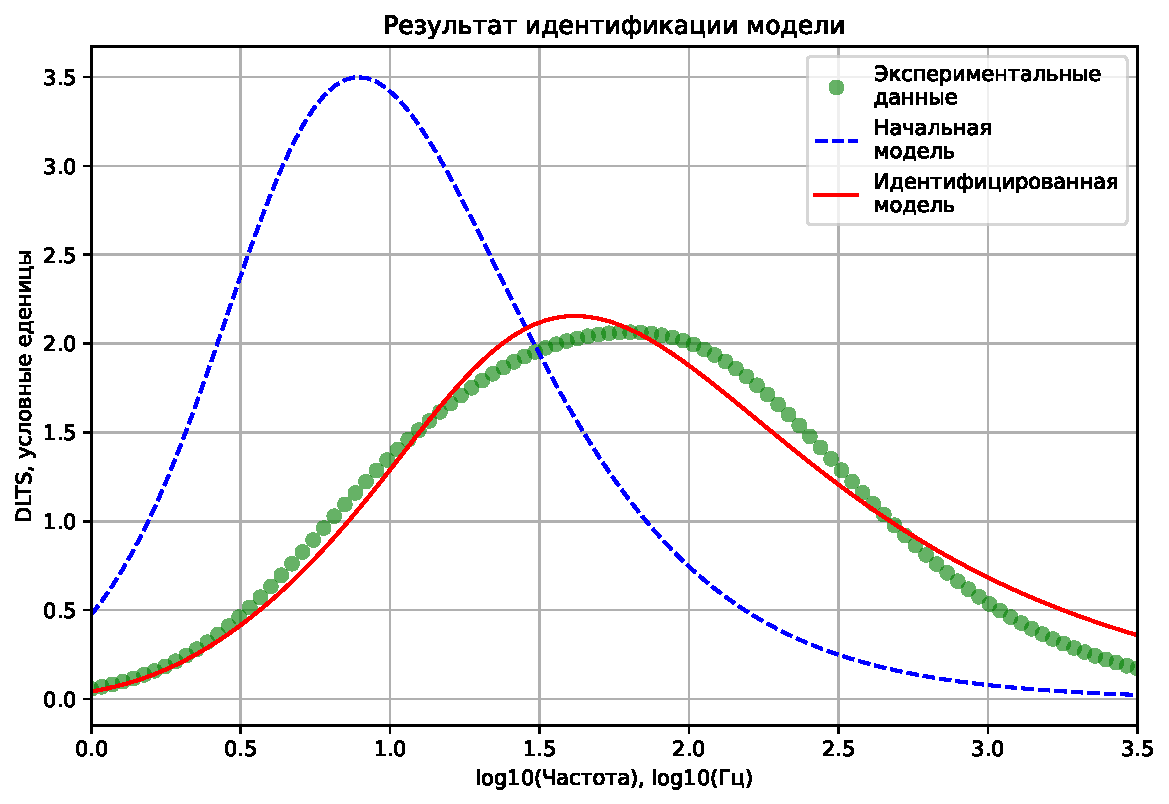
\includegraphics[width=\linewidth]{identification_results_17}
			\caption{Рассчитанный частотный скан и результаты идентификации}
			\label{pic:results_1_scan}
		\end{subfigure}
		\caption{Результаты моделирования частотного скана №18}
		\label{pic:result_1}
	\end{figure}

	\begin{figure}[h!]
		\centering
		\begin{subfigure}[c]{0.3\textwidth}
			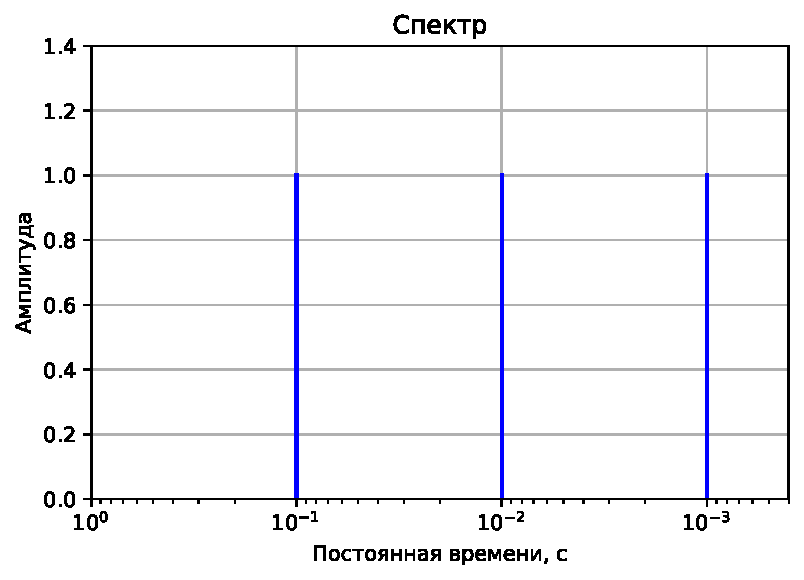
\includegraphics[width=\linewidth]{spectr30}
			\caption{Спектр}
			\label{pic:results_2_spectr}
		\end{subfigure}
		\begin{subfigure}[c]{0.45\textwidth}
			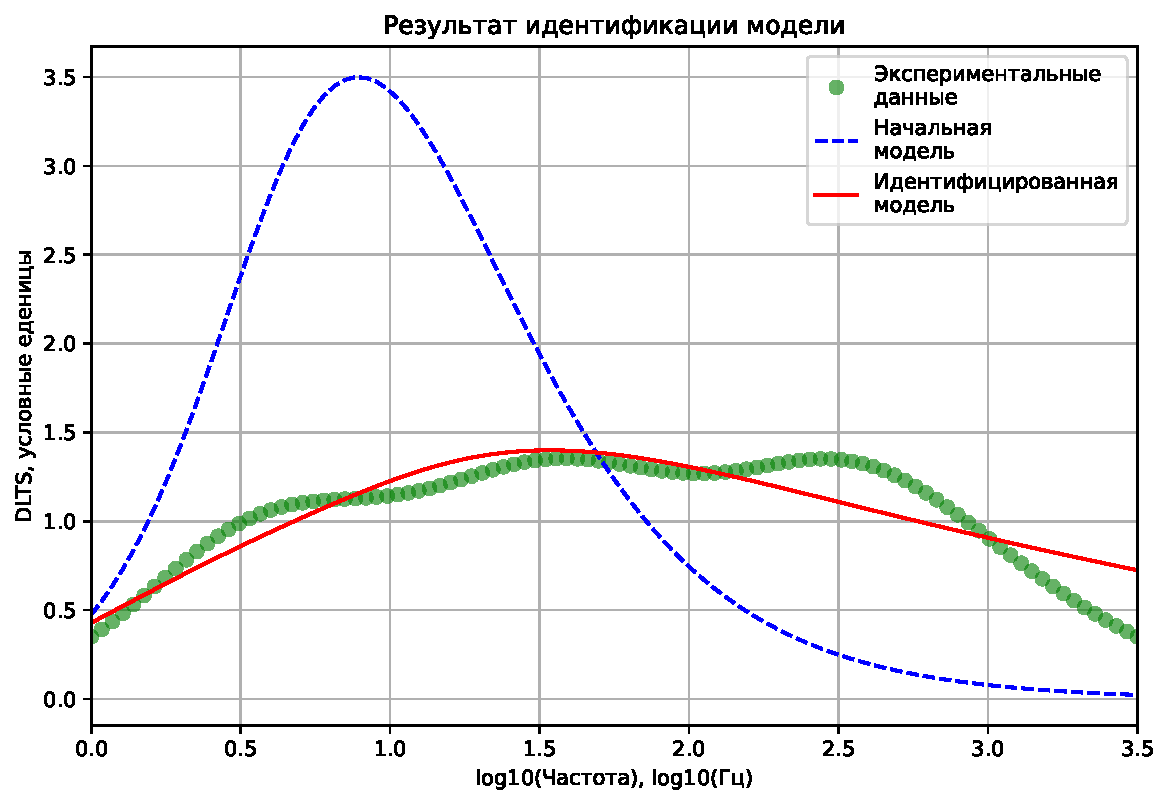
\includegraphics[width=\linewidth]{identification_results_30}
			\caption{Рассчитанный частотный скан и результаты идентификации}
			\label{pic:results_2_scan}
		\end{subfigure}
		\caption{Результаты моделирования частотного скана №31}
		\label{pic:result_2}
	\end{figure}

	\begin{figure}[h!]
		\centering
		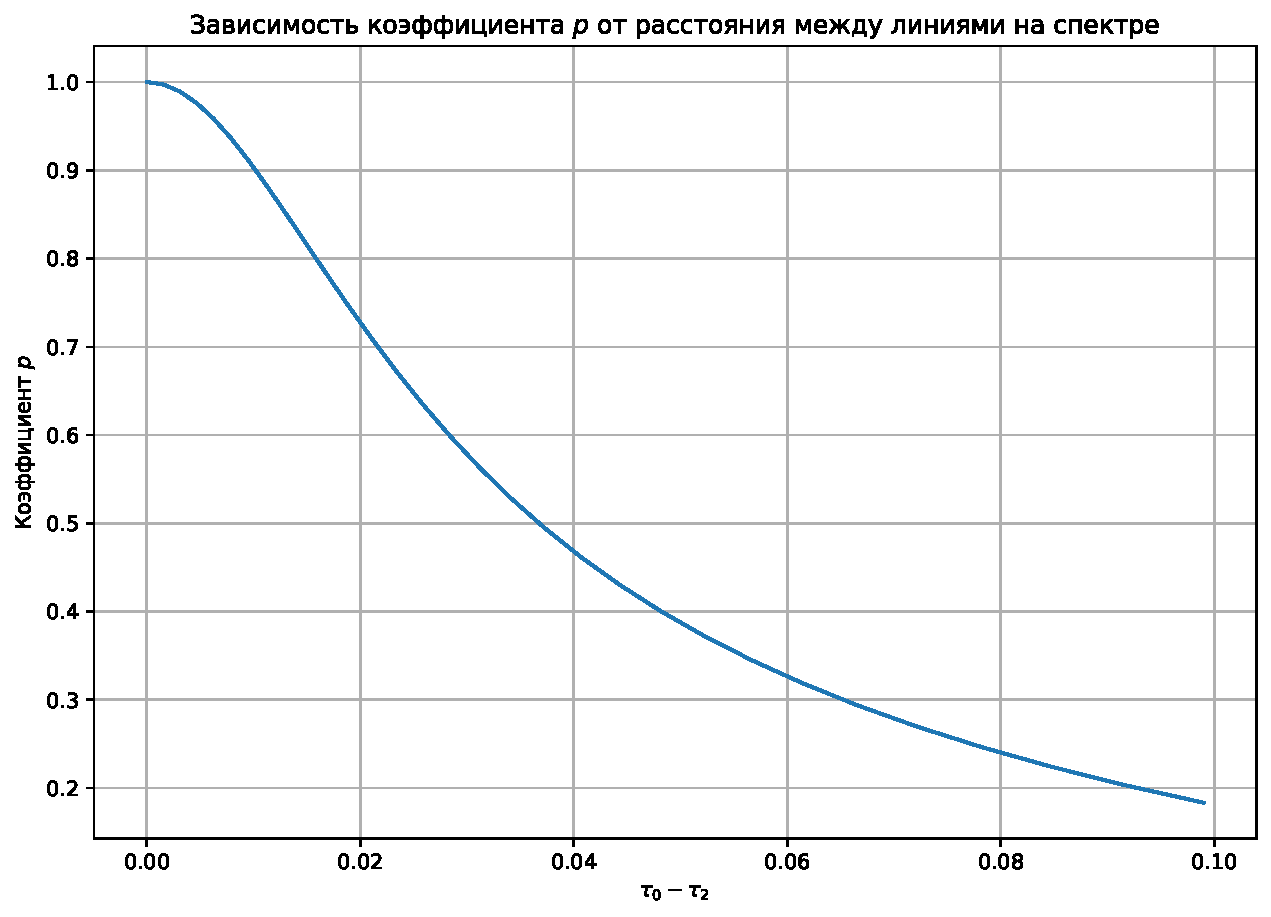
\includegraphics[width=0.7\textwidth]{semilogx_p_func}
		\caption{Зависимость показателя $p$ от разности постоянных времени
		крайних на спектре линий.}
		\label{pic:p_delta_tau}
	\end{figure}

    \section{Выводы}
	\begin{enumerate}
		\item Полученные результаты моделирования частотных сканов 
		(рисунок~\ref{pic:p_delta_tau}, таблица~\ref{table:results})
		позволяют сделать вывод о том, что коэффициент 
		нелинейности"=неэкспоненциальности $p$ нелинейно убывает с 
		увеличением разности постоянных времени крайних линий на спектре
		($\tau_0 - \tau_2$).
		\item С увеличение разности постоянных времени крайних линий на 
		спектре растёт среднеквадратическая ошибка между результатами,
		полученными на идентифицированной модели, и исходными данными.
		\item Возможно улучшение программной реализации модели и повышение
		скорости идентификации её параметров.
	\end{enumerate}

    % \pagebreak
    
    \printbibliography[heading=bibintoc]

    \pagebreak

    \section*{Приложение}
\addcontentsline{toc}{section}{Приложение 1}
	\begin{table}[ht]
	\begin{tabular}{|l|l|l|l|l|l|l|l|l|l|l|}
        \hline
		№  & $A$  & $\log10(\tau)$ & $p$   & $E$      & $\tau_0$ & $\tau_1$ & $\tau_2$ & $A_0, A_1, A_2$\\ \hline
		0  & 3    & -2             & 1     & 7.65E-10 & 0.01     & 0.01     & 0.01     & 1              \\ \hline
		1  & 3    & -2             & 0.999 & 3.04E-08 & 0.0104   & 0.01     & 0.00962  & 1              \\ \hline
		2  & 3    & -2             & 0.997 & 4.73E-07 & 0.0108   & 0.01     & 0.00926  & 1              \\ \hline
		3  & 2.99 & -2             & 0.994 & 2.38E-06 & 0.0112   & 0.01     & 0.00891  & 1              \\ \hline
		4  & 2.98 & -2             & 0.989 & 7.47E-06 & 0.0117   & 0.01     & 0.00858  & 1              \\ \hline
		5  & 2.97 & -2             & 0.984 & 1.81E-05 & 0.0121   & 0.01     & 0.00825  & 1              \\ \hline
		6  & 2.96 & -2             & 0.976 & 3.71E-05 & 0.0126   & 0.01     & 0.00794  & 1              \\ \hline
		7  & 2.95 & -2             & 0.968 & 6.78E-05 & 0.0131   & 0.01     & 0.00764  & 1              \\ \hline
		8  & 2.93 & -2             & 0.959 & 0.000114 & 0.0136   & 0.01     & 0.00736  & 1              \\ \hline
		9  & 2.92 & -2             & 0.948 & 0.00018  & 0.0141   & 0.01     & 0.00708  & 1              \\ \hline
		10 & 2.9  & -2             & 0.937 & 0.000269 & 0.0147   & 0.01     & 0.00681  & 1              \\ \hline
		11 & 2.88 & -2             & 0.924 & 0.000386 & 0.0153   & 0.01     & 0.00656  & 1              \\ \hline
		12 & 2.85 & -2             & 0.911 & 0.000535 & 0.0158   & 0.01     & 0.00631  & 1              \\ \hline
		13 & 2.83 & -2             & 0.897 & 0.000719 & 0.0165   & 0.01     & 0.00607  & 1              \\ \hline
		14 & 2.81 & -2             & 0.882 & 0.000943 & 0.0171   & 0.01     & 0.00584  & 1              \\ \hline
		15 & 2.78 & -2             & 0.866 & 0.00121  & 0.0178   & 0.01     & 0.00562  & 1              \\ \hline
		16 & 2.75 & -2             & 0.85  & 0.00152  & 0.0185   & 0.01     & 0.00541  & 1              \\ \hline
		17 & 2.72 & -2             & 0.834 & 0.00188  & 0.0192   & 0.01     & 0.00521  & 1              \\ \hline
		18 & 2.69 & -2             & 0.817 & 0.00229  & 0.02     & 0.01     & 0.00501  & 1              \\ \hline
		19 & 2.66 & -2             & 0.799 & 0.00274  & 0.0207   & 0.01     & 0.00482  & 1              \\ \hline
		20 & 2.63 & -2             & 0.781 & 0.00325  & 0.0215   & 0.01     & 0.00464  & 1              \\ \hline
		21 & 2.6  & -2             & 0.763 & 0.00381  & 0.0224   & 0.01     & 0.00447  & 1              \\ \hline
		22 & 2.57 & -2             & 0.745 & 0.00441  & 0.0233   & 0.01     & 0.0043   & 1              \\ \hline
		23 & 2.53 & -1.99          & 0.727 & 0.00506  & 0.0242   & 0.01     & 0.00414  & 1              \\ \hline
		24 & 2.5  & -1.99          & 0.708 & 0.00574  & 0.0251   & 0.01     & 0.00398  & 1              \\ \hline
		25 & 2.47 & -1.99          & 0.69  & 0.00647  & 0.0261   & 0.01     & 0.00383  & 1              \\ \hline
		26 & 2.43 & -1.99          & 0.671 & 0.00723  & 0.0271   & 0.01     & 0.00369  & 1              \\ \hline
		27 & 2.4  & -1.99          & 0.653 & 0.00803  & 0.0282   & 0.01     & 0.00355  & 1              \\ \hline
		28 & 2.36 & -1.99          & 0.635 & 0.00884  & 0.0293   & 0.01     & 0.00341  & 1              \\ \hline
		29 & 2.33 & -1.99          & 0.616 & 0.00968  & 0.0304   & 0.01     & 0.00329  & 1              \\ \hline
		30 & 2.29 & -1.98          & 0.598 & 0.0105   & 0.0316   & 0.01     & 0.00316  & 1              \\ \hline
	\end{tabular}
\end{table}
    В таблице \ref{table:results} использованы следующие обозначения:
    \begin{description}
    	\item[$\tau_0, \tau_1, \tau_2$] -- Заданные постоянные времени
    	экспоненциальных составляющих на спектре в секундах.
    	\item[$A_0, A_1, A_2$] -- Заданные амплитуды экспоненциальных 
        составляющих на спектре в условных единицах. В данном случае 
        амплитуды всех составляющих равны 1.
    	\item[$p$] -- коэффициент нелинейности"=неэкспоненциальности,
    	полученный в результате идентификации параметров модели. 
        Безразмерная величина.
    	\item[$\tau$] -- постоянная времени, полученная в результате
    	идентификации параметров модели, в секундах.
    	\item[$A$] -- амплитуда, полученная в результате идентификации
    	параметров модели, в условных единицах.
    	\item[$E$] -- среднеквадратическая ошибка (квадрат единиц 
        амплитуды $A$).
    \end{description}

\end{document}